% Chapter Template

\chapter{Angular} % Main chapter title

\label{Chapter4} % Change 4 to a consecutive number; for referencing this chapter elsewhere, use \ref{Chapter4}

\section{Definition}

Angular is a JavaScript framework for developing client side applications. This framework was created on October 2010 by Google. It is maintained by Google and a community of individual developers since September 2016 that its code became open source. (\cite{Reference6}) Angular as framework is providing a large set of libraries, functions and tools, and its implementing the entire structure of a client-side application. Moreover, Angular is using templates that extend HTML style syntax for view's representation, and is built in TypeScript, a JavaScript-like language. (\cite{Reference19}) \par

Angular's advantage is that provides the ability of creating and managing project through terminal. Due to its complicated set up, Google created a command line interface, or CLI, that makes Angular's usage much easier. Angular CLI is responsible for creating and maintaining common pattern inside an app. (\cite{angularUpandRunning}) Creating projects, adding new controllers and much more other tasks, are automated and easy implemented with just one command. Last but not least, Angular CLI is based on Webpack, a tool that groups TypeScript, JS, CSS, HTML and any files used in the application, and makes deployment, building app for production, simpler. (\cite{murray2018ng}) \par

\subsection{Angular \& AngularJS}

AngularJS, or sometimes referred as Angular 1, was firstly released in order to provide quick, scalable and maintainable web applications. As years passed, the way browsers, and generally web, used to work changed dramatically, so AngularJS stopped solving problems relevant with the new updates of web. Thus, Angular was created on 2014 which is basically a totally newly written framework. As "Angular" are referred all the newest version, starting from Angular2 and above.(\cite{angularUpandRunning}) \par

More specifically, Angular and AngularJS are two different frameworks made from the same team. As regards AngularJS, it is using directives, controllers, scopes, services and dependency injections, while Angular is using components, instead of directives, and services. Comparing these two frameworks, modules were replaced by web components and existing features of AngularJS were improved, such as dependency injection and templating. (\cite{angularUpandRunning}) Scope, which stands for two-way binding, and directive definition objects, controllers and angular.module were removed from the new versions of Angular. (\cite{murray2018ng}) \par

\subsection{HTTP}

Angular is providing an impended HTTP library through which external APIs can be called. The HTTP requests made are asynchronous that enhance pages performance. This means that user can continue interacting without waiting for the HTTP's response. In general, there are three ways of dealing with asynchronous code in Angular, Callbacks, Promises and Observables. (\cite{murray2018ng})

\subsection{Testing}

When using Angular CLI for component's creation, its main infrastructure is set up and includes four files. One file is for writing css, one for html, one for TypeScript code and one extra file for testing TypeScript code with a spec skeleton. There are some basic testing when initializing the component that can be improved and contain all test's needed for checking code's validation. (\cite{angularUpandRunning}) \par

\section{Typescript}

\begin{wrapfigure}[12]{r}{0.3\textwidth}
	\begin{center}
		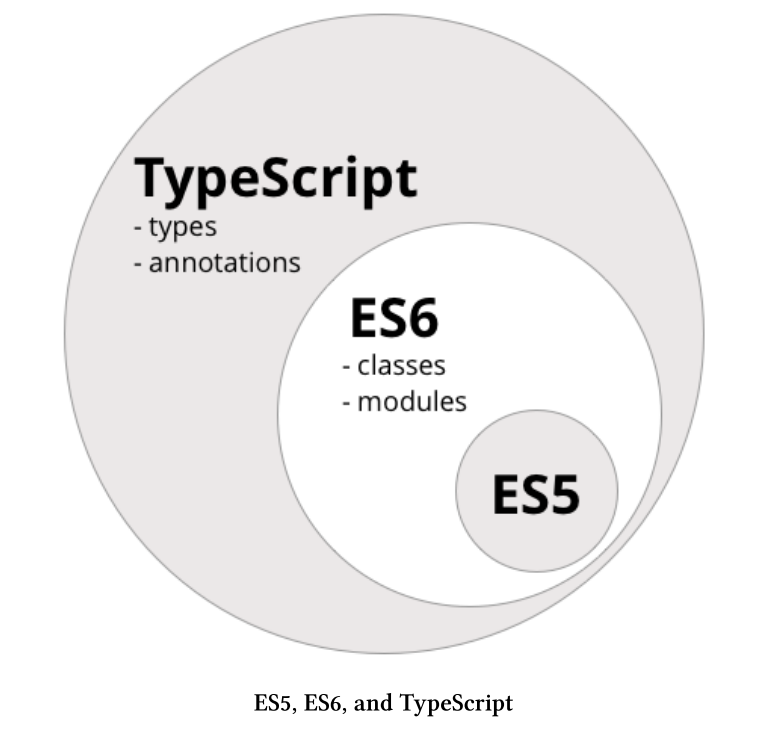
\includegraphics[scale=0.25]{images/Typescript.png}
	\end{center}
	\caption{Typescript}
\end{wrapfigure}

Angular is using a JavaScript-based language named TypeScript, which was the result of Microsoft's and Google's collaboration. TypeScript is a superset of ES6 with the additional features of types and annotations, as it is shown in the diagram bellow. It is compiled to ES5 in order code to be compatible with browsers, but it have five major upgrades compared to ES5 code that will be described later on this section. (\cite{murray2018ng}) \par

It is not obligatory to write TypeScript in Angular apps. However, it is a good practice due to the features provided, that also make coding easier to be maintained and understood. (\cite{angularUpandRunning}) \par

\subsection{Types}

TypeScript's name was inspired by its typing system, its most important addition. Type checking can prevent developers from bugs and make code much readable due to its obligatory clarification. (\cite{murray2018ng}) \par 

Regarding types provided, they are the same as in JavaScript, booleans (true or false), numbers, strings, arrays, enums (similar to arrays but has numeric values as names), any (any type of value), void (no type or returned value expected). Types are not necessarily used in TypeScript, they can be omitted in case of writing quick code. (\cite{murray2018ng}) \par
decorator
\subsection{classes} 


ES5 JavaScript is using functions and prototype-based objects, through which an object-oriented approach is succeed. In this version, prototypes are used instead of classes. (\cite{murray2018ng}) In contrast, ES6 version is using an object-oriented approach based on classes, that inherit functionality and built objects. (\cite{Typescript}) \par

In more details, classes include properties, methods and constructors. Properties are the data passed as arguments to a class's instance and can also refer to a type. A regards methods, they are functions included in an object and are called through the instances of them. Lastly, every object owns at least one constructor, which is a method executed at the creation of class's instance. It can take parameters, but it does not return any values except the instance of the object. As object-oriented, classes inherit their behavior from their parent which can be then modified. (\cite{murray2018ng}) \par

\subsection{Imports}

By using import, library modules and other Angular applications are imported in components, services and other parts of the application. In this way, functionalities included in these imports can be used, and extra both code and effort by developer's side can be reduced. (\cite{angularUpandRunning})

\subsection{Decorators}

With the introduction of Classes in TypeScript and ES6, there now exist certain scenarios that require additional features to support annotating or modifying classes and class members. Decorators provide a way to add both annotations and a meta-programming syntax for class declarations and members. Decorators are a stage 2 proposal for JavaScript and are available as an experimental feature of TypeScript. (\cite{Typescript})

A Decorator is a special kind of declaration that can be attached to a class declaration, method, accessor, property, or parameter. Decorators use the form @expression, where expression must evaluate to a function that will be called at runtime with information about the decorated declaration. (\cite{Typescript})

\subsection{Utilities}

Due to TypeScript is a superset of ES6 JavaScript, extended syntax feature of ES6 are also included in TypeScript and make programming easier. First of all, arrow functions is an important addition. Generally, the arrow-syntaxed functions are sharing the same this with the rest of their component or service. In contrast, when a function is applied in traditional JS, it gives its own this, fact that leads to difficulties using global variables and functions. Moreover, new template string were added, thus variables can be included in strings, as long as backticks are used instead of double or single quotes, and multi-line strings are allowed. (\cite{murray2018ng}) \par

\section{Components}

Angular components are TypeScript classes decorated with extra attributes and meta-data. Classes basically include any data and functionality needed, whereas decorators define the way of translating to HTML. (\cite{angularUpandRunning}) \par

Angular applications are in fact a tree of components, where its root is the application and that's what it will be rendered when any updates exist. As regarding components, they can be built from smaller components that consist of parent-child structure. When a component is rendered in Angular, its dependent components are updated as well. (\cite{murray2018ng}) \par

More specifically, components have three main parts, which are component's decorator or @Component, a view and a controller. Each component is responsible for a small part of screen and controls this part through templates. Component's decorator is responsible for defining to other parts of the application how interaction with the component is succeeded. For this purpose, it uses templates, which is the visual part of component or as called the view, and selectors, which indicates how components will be recognized from templates and what parts of HTML match the component. As regards controllers, they accept server's requests and run comprehensive actions based on paths and parameters sent by server. These actions are responsible for rendering components when needed. (\cite{murray2018ng}) \par

\section{Services}

In Angular, components are responsible for data representation and user interface's updates. Data are passed from components to the screen and, through events, from screen to component's methods where changes for user interface  will be handled. Basically, components is the presentation layer, while servers are the ones responsible for fetching real data and business logic to the application. (\cite{murray2018ng}) \par

More specifically, Angular services are a common layer through the application that is used in three cases. Firstly, services are created when data are needed from or sent to the server. Secondly, services can be applied for writing application logic that can be reused across components. Additionally, services are used in case data sharing via components, particularly when components do not have access to one another. (\cite{angularUpandRunning}) \par

Services have their own store and can access all components in the application. Generally, they are the layer that handles how data and application logic works, so as components to be only bound to what will be represented in screen. (\cite{angularUpandRunning}) \par

\section{Lifecycle Methods}

Each component and directive has its life-cycle that is handled by Angular. Angular's lifecycle hooks were created in order developers to write code that acts at specific moments of directive's or component's life. Life-cycle hooks are provided through an interface in each part of the app needed. There are three main stages of life-cycle, creation, update and destruction, that each includes a list of hooks. In order to add these hooks in code, it is needed declaration of interface's implementation inside directive or component and also of hook's methods wanted. Hook methods are formed by the name of hook plus the prefix "ng". In this way, Angular will call the component or directive, and code written in methods at the right time. (\cite{murray2018ng}) \par

In figure 4.2, it is shown the process followed in the lifecycle of any Angular-based app.

\begin{figure}[h!]
	\begin{center}
		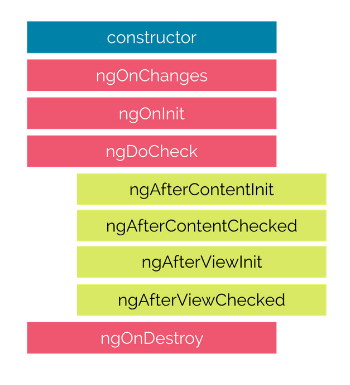
\includegraphics[scale=0.65]{images/Lifecycle-hooks_Angular.png}
	\end{center}
	\caption{Life-cycle hooks in Angular}
\end{figure}

Let's dive into hook methods represented in the diagram above. Constructor is the first method executed and includes any initializations needed. Afterwards, when values of properties or data are modified, ngOnChanges method is triggered. Method ngOnInit is following and is used to perform complicated initializations that cannot be made in constructor. (\cite{Reference19}) Every time data change all related components or directives are updated, fact that affects performance. So, in case that a change is not important to be executed or an update is needed when a specific property have been modified, onDoCheck method can be used. This method overrides ngOnChanges which is ignored. (\cite{murray2018ng}) Moving forward, ngAfterContentInit is triggered when content is extended into component's view, while ngAfterContentChecked when this content is checked after its projection. Furthermore, ngAfterViewInit is relevant only to components and called after the initialization of component's and its child's views. The same with ngAfterViewChecked method which is executed after the views are checked by Angular. Finally, ngOnDestroy is the method that clears up any data remained in directives or components before they are removed.(\cite{Reference19}) \par

It is not obligatory hooks to be implemented in a class, but it is considered as a good practice. Performance can be increased and actions in particular moments can be executed. (\cite{murray2018ng}) \par

\section{Two or one-way data binding}

Two-way data binding is an architecture in which information flows from state to view and vice versa. In Angular JS, the default data flow is the two-way binding, or MVW as noticed in \ref{Chapter2}, which means that when model is modified, view is also changed and the other way around. (\cite{murray2018ng}) This type of binding is easy to start with and is also suitable for totally interactive user interfaces since data are changed by two different directions. (\cite{Reference21}) \par

On the other hand, two direction data binding is possible to cause a flow of unpredictable updates and a difficulty to follow data flow as application goes bigger. Moreover, another problem with this architectural approach is that it binds data flow with DOM tree. For these reasons, new released Angular is flexible to change between one or two-way data structure if it is needed. As described in Chapter \ref{Chapter2}, two-direction binding pass data down via components and event handlers needed to reflect state based on view layer's changes. For adapting one-way structure, Angular can use either Observables-based, such as Reactive Extensions Library for JavaScript (RxJS), or Flux-based architecture, such as Redux. When using Observables as main data architecture in Angular, it is named Reacting Programming which is a way to use asynchronous data streams. (\cite{murray2018ng}) \par

\section{Summery}

Angular is a framework that includes most of libraries and functionalities needed to built a client-side application. Moreover, it is well combined with TypeScript language and is widely used by both individual developers and companies. In this chapter, was covered the definition and main functionality of Angular. \par

% 6 pages
